% Synchronized to r30323

\include{fli4l}
\makeindex

\begin{document}

\newcommand{\titlename}{Paquetage PROXY}

\flhypersetup{pdftitle=\titlename}
\pdfbkmrk{-1}{\titlename}{title}
\title{\titlename\\ Version \version}

\author{Frank Meyer\\ \email{frank@fli4l.de} \and L'équipe fli4l\\ \email{team@fli4l.de}}

\maketitle
\pdfbkmrk{0}{\contentsname}{table}
\tableofcontents

\chapter{Documentation du paquetage PROXY}
% Synchronized to r43697
\section {PROXY - Several Proxy Servers}

% subsections included in proxy.tex

% Synchronized to r43697
\subsection{OPT\_PRIVOXY - Filtrage de la publicité avec un proxy HTTP}
\configlabel{OPT\_PRIVOXY}{OPTPRIVOXY}

    Privoxy "Privacy Enhancing Proxy" (="filtrage avancé, pour la protection de
    la vie privée") voir le site Web officiel de Privoxy (\altlink{http://www.privoxy.org/}).
    Privoxy filtre le contenu des pages web sur votre navigateur, en remplaçant
    par des images vides les bannières publicitaires et les Popups, Il gére les
    cookies dans une mémoire cache (petit paquet de données avec lesquels un site
    web peut reconnaître certain surfer) et empêche l'affichage de ce que l'on
    appelle bugs-Web (ce sont de grandes images 1x1 pixels, qui sont utilisées,
    pour espionner le comportement des utilisateurs sur le Net).

    Pendant que Privoxy fonctionne, vous pouvez tout simplement configurer et
    activer les paramètres par l'intermédiaire de l'interface Web. L'interface
    Web se trouve à l'adresse \altlink{http://config.privoxy.org/} ou en abrégée
    \altlink{http://p.p/}.

    \marginpar{Une configuration ainsi activer ne survit pas à un redémarrage
    du routeur fli4l\ldots (tobig)}

    Privoxy Internet Junkbusters à eu une évolution conséquente à partir de la
    version 2.1.0, voir le site Web (\altlink{http://www.junkbuster.com/}).
    L'innovation la plus importante, est que toutes les règles de filtrage sont
    centralisées dans un fichier \texttt{default.action}. Celui-ci se trouve dans le
    répertoire fli4l \texttt{/etc/privoxy}. Le grand avantage de cette méthode c'est
    que les nouvelles versions de ce fichier peuvent être télécharger séparément
    à cette adresse \\
    \altlink{http://sourceforge.net/projects/ijbswa/files/}.\\
    Ainsi, chaque utilisateur fli4l peut tenir ce fichier à jour, sans mettre
    à jour le routeur-fli4l. (Actuellement, la version 1.8 de ce fichier est
    dans ce paquetage)

\begin{description}
\config{PRIVOXY\_MENU}{PRIVOXY\_MENU}{PRIVOXYMENU}

        Avec cette variable, vous pouvez ajouter la section Privoxy au menu-httpd.

\config{PRIVOXY\_N}{PRIVOXY\_N}{PRIVOXYN}

        Vous indiquez dans cette variable le nombre de Privoxy qui doit être
        enregistré pour chaque interface.

\config{PRIVOXY\_x\_LISTEN}{PRIVOXY\_x\_LISTEN}{PRIVOXYxLISTEN}

        {Vous indiquez dans cette variable, l'adresse-IP ou le nom symbolique,
        y compris le numéro de Port de l'interface, sur lequel le Privoxy doit
        écouter les connexions des clients. C'est une bonne idée d'indiquer
        ici, seulement les adresses des interfaces que l'on fait confiance, car
        tous les ordinateurs auront un accès complet à travers le Privoxy (avec
        bien sur le navigateur configuré et activé). En règle générale il est
        judicieux d'indiquer, la valeur par défaut qui est \var{IP\_NET\_1\_IPADDR:8118}

        Avec l'adresse indiquée ici, le Privoxy écoute et offre ses services.
        Le port par défaut est 8118. Vous devez utiliser cette information pour
        configurer le proxy dans votre navigateur. Pour plus de détail sur
        la configuration d'Internet Explorer et de Netscape Navigator, voir le
        site Web~:

        \altlink{http://www.privoxy.org/} \marginpar{URL précise}

        Vous devez enregistrer dans chaque navigateur, en tant que proxy
        l'ordinateur-fli4l, vous allez donc prendre le nom de la variable
        HOSTNAME='fli4l' ou l'adresse-IP (par ex. 192.168.6.1) de la variable
        \var{HOST\_\-x\_\-IP}='192.168.6.1' qui est dans le fichier config de
        fli4l. Avec le Port par défaut, on a ici tous les paramètres nécessaires,
        pour configurer votre navigateur Web, pour l'utilisation du Privoxy.}

\config{PRIVOXY\_x\_ALLOW\_N}{PRIVOXY\_x\_ALLOW\_N}{PRIVOXYxALLOWN}

        {Vous indiquez dans cette variable le nombre d'adresse réseau à installer.}

\config{PRIVOXY\_x\_ALLOW\_x}{PRIVOXY\_x\_ALLOW\_x}{PRIVOXYxALLOWx}

        Vous indiquez dans cette variable l'adresse réseau ou l'adresse-IP pour
        le quelle le filtrage de paquets doit être ouvert. Normalement il est
        logique d'indiquer ici le paramètre \var{IP\_NET\_1}.

\config{PRIVOXY\_x\_ACTIONDIR}{PRIVOXY\_x\_ACTIONDIR}{PRIVOXYxACTIONDIR} {

  Avec cette variable vous indiquez l'emplacement, ou vous pouvez paramétrer
  l'ensembles des règles Privoxy (pour les fichiers \emph{default.action} et
  \emph{user.action}) sur le routeur. Le chemin d'accès spécifié est évaluée par
  rapport au répertoire racine. Cette variable peut être utilisé pour deux
  choses différentes~:

\begin{description}
  \item [Le déplacement dans la mémoire permanente de l'ensemble des règles]
  Si vous spécifiez un répertoire dans un emplacement autre que le disque-RAM,
  au démarrage de fli4l l'ensemble des règles défini par défaut seront copiés et
  utilisé à partir de cet emplacement. Les modifications apportées à ces
  ensembles de règles survivront à un redémarrage du routeur. On doit aussi
  tenir compte du fait qu'après une mise à jour du paquetage Privoxy, ces règles
  seront toujours utilisées donc l'ensemble des règles du paquetage de mise à
  jour sera simplement ignoré.
  \item [l'utilisation de vos propres ensembles de règles]
  L'utilisateur fli4l permet d'écrire des règles spécifiques à la place des
  règles standard. Vous devez dans cette variable indiquer votre propre
  sous-répertoire qui sera dans le répertoire \emph{config} (par exemple
  \emph{etc/mon\_privoxy}, par contre vous ne devez pas indiquer \emph{etc/privoxy})
  ensuite vous placez dans ce sous-répertoire vos propres règles.
\end{description}

         Le paramétrage de cette variable est optionnel.}

\config{PRIVOXY\_x\_HTTP\_PROXY}{PRIVOXY\_x\_HTTP\_PROXY}{PRIVOXYxHTTPPROXY}

        {Si vous voulez utiliser en plus du Privoxy un autre Proxy HTTP,
        c'est-à-dire utiliser également des pages Web en cache, vous pouvez
        paramétrer cette variable. Le Privoxy utilise alors ce proxy. Avec cette
        variable vous avez l'avantage utilisé plusieurs Proxys. Le paramètre
        peut ressembler à cela~:

\begin{example}
\begin{verbatim}
        PRIVOXY_1_HTTP_PROXY='mon.provider.de:8000'
\end{verbatim}
\end{example}
        Ce paramètre est optionnel.}

\config{PRIVOXY\_x\_SOCKS\_PROXY}{PRIVOXY\_x\_SOCKS\_PROXY}{PRIVOXYxSOCKSPROXY}

        {Si vous voulez utiliser en plus du Privoxy un autre Proxy SOCKS. Pour
        augmenter la surveillance privée de la transmission de données du Privoxy,
        par exemple, envoyé les données par le réseau Tor, vous pouvez paramétrer
        cette variable. Pour plus de détails sur Tor, reportez-vous à la
        \jump{OPTTOR}{Documentation Tor}. Le paramètre pour utiliser Tor peut
        ressembler à cela~:

\begin{example}
\begin{verbatim}
        PRIVOXY_x_SOCKS_PROXY='127.0.0.1:9050'
\end{verbatim}
\end{example}
        Ce paramètre est optionnel.}

\config{PRIVOXY\_x\_TOGGLE}{PRIVOXY\_x\_TOGGLE}{PRIVOXYxTOGGLE}

        {Avec cette variable vous pouvez arrêter le proxy par l'interface Web.
        Si le Privoxy est mis hors circuit, il réagira simplement comme
        Proxy-Forwarding et ne modifiera plus le contenu des pages Web transférées.
        Vous devez considérer, que ce réglage vaut pour TOUS les utilisateurs du
        Proxy, c.-à-d. que si un utilisateur arrête Privoxy, le Privoxy sera coupé
        pour tous les autres utilisateurs Web qui transfert par le Proxy.}

\config{PRIVOXY\_x\_CONFIG}{PRIVOXY\_x\_CONFIG}{PRIVOXYxCONFIG}

        {Avec cette variable, les utilisateurs ont la possibilité de configurer
        le proxy par l'interface web. Pour plus de détails, je vous demande
        de consulter la documentation Privoxy qui est ici.}

\config{PRIVOXY\_x\_LOGDIR}{PRIVOXY\_x\_LOGDIR}{PRIVOXYxLOGDIR}

        {Dans cette variable vous pouvez indiquer le répertoire du fichier log
        (ou journal) pour le privoxy. Cela peut être utile, par ex. lorsque
        l'utilisateur veut enregistrer les accès des sites Web. Si rien n'est
        spécifié (par défaut), les principaux messages seront enregistrés sur l
        console, de plus la variable \var{PRIVOXY\_\-LOGLEVEL} sera ignorée.}

        Vous pouvez aussi indiquer 'auto', le chemin du fichier log sera alors
        déplacé dans le répertoire système, pour avoir des données persistantes.
        S'il vous plaît, assurez-vous que la variable \var{FLI4L\_UUID} soit dans
        ce cas configuré correctement. Comme on peut si attendre une grandes
        quantités de données sera enregistrées et le fichier log dans le /boot
        ou dans le Disque-RAM sera rempli rapidement.

\config{PRIVOXY\_x\_LOGLEVEL}{PRIVOXY\_x\_LOGLEVEL}{PRIVOXYxLOGLEVEL}

        {On indique dans cette variable les valeurs, pour que Privoxy puisse
        enregistrer les événements dans le fichier log. Il est possible d'ajouter
        plusieurs valeurs à la suite, vous devez les séparer par un espace. Les
        valeurs suivantes peuvent être ajoutées.

        \begin{tabular}[h!]{rl}

    Valeur & ce qui sera enregistré~? \\
    \hline
    1    & Chaque Requête (GET/POST/CONNECT). \\
    2    & Le statut de chaque connexion \\
    4    & Le statut-I/O \\
    8    & Header-Parsing \\
    16   & \textbf{Toutes} les données \\
    32   & Debug force-feature \\
    64   & Debug regular expression filters \\
    128  & Debug redirects \\
    256  & Debug GIF animation \\
    512  & Common Log Format (Analyse fichier-log) \\
    1024 & Debug kill pop-ups \\
    2048 & CGI (server web) user interface \\
    4096 & Startup banner and warnings \\
    8192 & Non-fatal errors \\
        \end{tabular}

        Pour produire un fichier log (ou journal) avec Common Log Format, vous
        devez indiquer SEULEMENT la valeur 512, si vous indiquez d'autres
        valeurs le fichier log sera "pollué" par d'autres enregistrements
        et vous aurez des problèmes pour l'analyser.}
\end{description}

        Privoxy offre de très nombreuses options de configurations. Cependant
        pour des raisons compréhensibles nous ne pouvons pas développer toutes
        ces options dans le fichier de configuration de fli4l. Beaucoup de ces
        options peuvent être paramétrées sur l'interface Web de Privoxy. Vous
        trouverez des infos plus précises pour la configuration de ces fichiers
        sur la page d'accueil de Privoxy. Les fichiers de configuration de
        Privoxy se trouvent dans le répertoire $<$fli4l-Version$>$/opt/etc/privoxy/.
        Ce sont des fichiers originaux du Paquetage-Privoxy, toutefois, pour
        gagner de la place, tous les commentaires ont été supprimés.

% Synchronized to r43697
\subsection{OPT\_TOR - Système de communication anonyme pour Internet}
\configlabel{OPT\_TOR}{OPTTOR}

Tor est l'outil d'un grand nombre d'organismes et de simples citoyens, qui
veulent améliorer leur protection et leur sécurité sur Internet. L'utilisation
de Tor vous aide à être anonymes lors de la navigation et de la publication sur
le Web, messagerie instantanée, IRC, SSH et autres applications basées sur TCP.
En outre, Tor fournit une plate-forme sur laquelle les développeurs de logiciels
peuvent créer de nouvelles applications pour plus d'anonymat, sur la sécurité et
la protection de la vie privée.

\altlink{https://www.torproject.org/index.html.fr}

\begin{description}
\config{TOR\_LISTEN\_N}{TOR\_LISTEN\_N}{TORLISTENN}

\config{TOR\_LISTEN\_x}{TOR\_LISTEN\_x}{TORLISTENx}

        {Dans la première variable, vous indiquez le nombre d'adresse réseau,
        dans la deuxième variable vous indiquez l'adresse-IP ou le nom symbolique,
        y compris le numéro de Port de l'interface, sur lequel Tor doit écouter
        les connexions des Clients. C'est une bonne idée, d'indiquer ici seulement
        les adresses des interfaces que l'on fait confiance, car tous les
        ordinateurs auront un accès complet à travers Tor (avec bien sur le
        navigateur configuré et activé). En règle générale il est judicieux
        d'indiquer, la valeur par défaut qui est \var{IP\_NET\_1\_IPADDR:9050}

        Avec l'adresse indiquée ici, Tor écoute et offre ses services. Le port
        par défaut est 9050. Vous devez utiliser cette information pour
        configurer le proxy dans votre navigateur.

        Vous devez indiquer dans chaque navigateur en tant que proxy
        l'ordinateur-fli4l, vous allez donc prendre le nom de la variable
        HOSTNAME='fli4l' ou l'adresse-IP (par ex. 192.168.6.1) de la variable
        \var{HOST\_\-x\_\-IP}='192.168.6.1' qui est dans le fichier config de
        fli4l. Avec le Port par défaut, on a ici tous les paramètres nécessaires,
        pour configurer votre navigateur Web, pour l'utilisation de Tor.}

\config{TOR\_ALLOW\_N}{TOR\_ALLOW\_N}{TORALLOWN}

        {Vous indiquez dans cette variable le nombre d'adresse réseau à installer.}

\config{TOR\_ALLOW\_x}{TOR\_ALLOW\_x}{TORALLOWx}

        Vous indiquez dans cette variable l'adresse réseau ou l'adresse-IP pour
        le quelle le filtrage de paquets doit être ouvert. Normalement il est
        logique d'indiquer ici le paramètre \var{IP\_NET\_1}.

\config{TOR\_CONTROL\_PORT}{TOR\_CONTROL\_PORT}{TORCONTROLPORT}

        Vous indiquez dans cette variable, le port TCP que Tor doit utiliser,
        pour le contrôle d'accès via le protocole Tor. Cette variable
        est optionnelle, si rien n'ai indiqué cette fonction sera désactivée.

\config{TOR\_CONTROL\_PASSWORD}{TOR\_CONTROL\_PASSWORD}{TORCONTROLPASSWORD}

        Vous spécifier dans cette variable, un mot de passe pour le contrôle
        d'accés.

\config{TOR\_DATA\_DIR}{TOR\_DATA\_DIR}{TORDATADIR}

        Cette variable est optionnelle. Si rien n'est indiqué, le dossier par
        défaut /etc/tor est utilisé.

\config{TOR\_HTTP\_PROXY}{TOR\_HTTP\_PROXY}{TORHTTPPROXY}

        {Si vous voulez utiliser en plus de Tor un autre Proxy http, Tor pourra
        alors utiliser ce proxy. Avec cette variable vous avez l'avantage utilisé
        plusieurs Proxys. Le paramètre peut ressembler à cela~:

\begin{example}
\begin{verbatim}
        TOR_HTTP_PROXY='mein.provider.de:8000'
\end{verbatim}
\end{example}

        Ce paramètre est optionnel.}

\config{TOR\_HTTP\_PROXY\_AUTH}{TOR\_HTTP\_PROXY\_AUTH}{TORHTTPPROXYAUTH}

        Une authentification peut-être nécessaire, vous devez la spécifier
        dans cette variable. Ainsi le mandataire sera enregistré sous la forme
        Nom d'utilisateur:Mot de passe.

\config{TOR\_HTTPS\_PROXY}{TOR\_HTTPS\_PROXY}{TORHTTPSPROXY}

        Vous pouvez enregistrer dans cette variable, un Proxy-HTTPS. Voir
        \smalljump{TORHTTPPROXY}{\var{TOR\_HTTP\_PROXY}}.

\config{TOR\_HTTPS\_PROXY\_AUTH}{TOR\_HTTPS\_PROXY\_AUTH}{TORHTTPSPROXYAUTH}

        Voir pour ce sujet \smalljump{TORHTTPPROXYAUTH}{\var{TOR\_HTTP\_PROXY\_AUTH}}.

\config{TOR\_LOGLEVEL}{TOR\_LOGLEVEL}{TORLOGLEVEL}

        {On indique dans cette variable les valeurs pour que Tor puisse
        enregistrer les événements dans le fichier log. Les valeurs suivantes
        sont possibles~: debug, info, notice, warn ou err. Les valeurs debug et
        info ne devraient pas si possible être utilisées, pour des raisons
        de sécurité.}

\config{TOR\_LOGFILE}{TOR\_LOGFILE}{TORLOGFILE}

        Si vous voulez utiliser un autre système que syslog pour enregistrer
        les événements de Tor, vous devez l'indiquer dans cette variable.

        Vous pouvez aussi indiquer 'auto', le chemin du fichier log sera alors
        déplacé dans le répertoire système, pour avoir des données persistantes.
        S'il vous plaît, assurez-vous que la variable \var{FLI4L\_UUID} soit dans
        ce cas configuré correctement. Comme on peut si attendre une grandes
        quantités de données sera enregistrées et le fichier log dans le /boot
        ou dans le Disque-RAM sera rempli rapidement.
\end{description}

% Last Update: $Id$
\subsection{OPT\_SS5 - Ein Socks4/5 Proxy}
\configlabel{OPT\_SS5}{OPTSS5}

Für einige Programme wird ein Socks-Proxy benötigt. SS5 stellt diese
Funktionalität bereit.

\altlink{http://ss5.sourceforge.net/}

\begin{description}

\config{SS5\_LISTEN\_N}{SS5\_LISTEN\_N}{SS5LISTENN}

\config{SS5\_LISTEN\_x}{SS5\_LISTEN\_x}{SS5LISTENx}

        {Hier werden die IP-Adressen oder symbolischen Namen inklusive
        der Portnummer der Interfaces angegeben, auf denen SS5 auf
        Verbindungen von Clients horchen soll. Es ist eine gute Idee,
        hier nur die Adressen der Interfaces anzugeben, denen man
        vertraut, da alle Rechner vollen Zugriff auf SS5 haben
        (und auf den eventuell aktivierten Konfigurations-Editor). In
        der Regel ist die Vorgabe \var{IP\_NET\_1\_IPADDR:8050}
        sinnvoll.

        Auf hier angegebenen Adressen lauscht SS5 und bietet seine
        Dienste an.  8050 ist der Standard-Port. Die Angabe hier muss
        man dann bei der Proxy-Konfiguration des jeweils verwendeten
        Programms benutzen.

        Als Proxy beim jeweiligen Programm muss der fli4l-Rechner
        angegeben werden, also das, was man bei HOSTNAME='fli4l'
        angegeben hat bzw.  dessen IP (z.B 192.168.6.1), die man bei
        \var{HOST\_\-x\_\-IP}='192.168.6.1' angegeben hat. Zusammen
        mit dieser Port-Angabe hier hat man dann alle nötigen Daten,
        um sein Programm für die Nutzung von SS5 zu
        konfigurieren.}

\config{SS5\_ALLOW\_N}{SS5\_ALLOW\_N}{SS5ALLOWN}

        {Gibt die Anzahl der Listeneinträge an.}

\config{SS5\_ALLOW\_x}{SS5\_ALLOW\_x}{SS5ALLOWx}

        Die Liste der Netze und/oder IP-Adressen für die der
        Paketfilter geöffnet wird. Sinnvoll ist hier auch wieder die
        Vorgabe \var{IP\_NET\_1}.

\end{description}



% Synchronized to r43697
\subsection{OPT\_TRANSPROXY (Expétimental) - Proxy HTTP transparent}
\configlabel{OPT\_TRANSPROXY}{OPTTRANSPROXY}

Transproxy est un proxy "transparent", c'est une application qui permet,
d'intercepter toutes les requêtes-HTTP qui passent par le routeur et de
les transmettre à un Proxy-HTTP normal, par ex. au Privoxy. Pour parvenir
à cette fonctionnalité, le filtre de paquets des requêtes HTTP qui doit
aller sur Internet, passent par le transproxy celui-ci les traite et les
transmet à un Proxy-HTTP. Iptables supporte cette fonction en utilisant
le paramètre "REDIRECT"~:

\begin{verbatim}
        PF_PREROUTING_1='tmpl:http IP_NET_1 REDIRECT:8081'
\end{verbatim}

Cette règle transmet tous les paquets-HTTP du premier réseau défini
(normalement c'est le LAN interne) au transproxy par le port 8081.

\begin{description}
\config{TRANSPROXY\_LISTEN\_N}{TRANSPROXY\_LISTEN\_N}{TRANSPROXYLISTENN}
\config{TRANSPROXY\_LISTEN\_x}{TRANSPROXY\_LISTEN\_x}{TRANSPROXYLISTENx}

        {Vous indiquez ici, les adresses IP ou les noms symboliques, ainsi
        que le numéro de port des interfaces, sur lesquels Transproxy doit
        écouter les connexions des clients. Si Toutes les interfaces spécifiées
        ici, utilise déjà un filtrage de paquets, Transproxy sera gêné
        par les paquets qui provient de ce filtrage. Avec la configuration
        par défaut \var{any:8081} Transproxy écoutera toutes les interfaces.}

\config{TRANSPROXY\_TARGET\_IP}{TRANSPROXY\_TARGET\_IP}{TRANSPROXYTARGETIP}
\config{TRANSPROXY\_TARGET\_PORT}{TRANSPROXY\_TARGET\_PORT}{TRANSPROXYTARGETPORT}

        {Grâce à cette option vous définissez le service pour lequel les requêtes
        HTTP doivent être redirigé. Cela peut être n'importe quel proxy standard
        HTTP (Squid, Privoxy, Apache, etc) et sur n'importe quel ordinateur (ou
        sur fli4l lui-même). Faire attention, que le Proxy ne se trouve pas dans
        le domaine du filtrage de paquet, dans lequel les requêtes http seront
        redirigées. Autrement un bouclage d'adresse apparaîtra.}

\config{TRANSPROXY\_ALLOW\_N}{TRANSPROXY\_ALLOW\_N}{TRANSPROXYALLOWN}
\config{TRANSPROXY\_ALLOW\_x}{TRANSPROXY\_ALLOW\_x}{TRANSPROXYALLOWx}

        {Liste des réseaux et/ou des adresses IP pour le filtrage de paquets
        ouvert. Cela devrait couvrir mêmes les réseaux, qui sont redirigés par
        le filtrage de paquets. Si aucun domaine n'est indiqué ici, vous devez
        indiquez les informations manuellement dans la configuration du filtrage
        de paquets.}
\end{description}

% Last Update: $Id$
\subsection{OPT\_SIPROXD (experimentell) -- Proxy für Session Initiation Protocol}
\configlabel{OPT\_SIPROXD}{OPTSIPROXD}

Möchte man mehrere SIP-Anwendungen (egal ob Ekiga, x-lite oder Hardware
SIP-Telefone) hinter einem Router betreiben, so kann es vorkommen,
dass Netzwerk-Ports speziell weitergeleitet werden müssen, da sonst
die Verbindungen nicht so funktionieren, wie sie sollten.

Um dies zu vermeiden, kann man einen speziellen SIP Proxy-Server nutzen.
Es werden derzeit (fli4l V4.0.0) mehrere solche Proxys evaluiert.
Sollte jemand über eine Empfehlung verfügen so darf er sich gerne
an das Team wenden!

% TODO  Den Einleitungstext an die tatsächlichen Gegebenheiten anpassen
%       (Siproxd implementiert, Kamailio nicht).

\subsubsection{Konfiguration}

\begin{description}

\config{SIPROXD\_N}{SIPROXD\_N}{SIPROXDN}

Gibt die Anzahl der Siproxd-Instanzen an, die gestartet werden sollen.
Mehrere Instanzen können nötig sein, wenn man SIP-Clients aus
verschiedenen hinter dem fli4l-Router liegenden Subnetzen benutzen will.

Standard-Einstellung: \verb+SIPROXD_N='0'+

Beispiel: \verb+SIPROXD_N='2'+

\config{SIPROXD\_x\_DEV\_IN}{SIPROXD\_x\_DEV\_IN}{SIPROXDxDEVIN}

Hier ist die Netzwerk-Schnittstelle zum lokalen Netz bzw. LAN hin
anzugeben, vom dem aus sich die VoIP-Clients mit dem SIP-Server
verbinden.  Erlaubt sind sowohl Namen von Netzwerkinterfaces (inklusive
VLAN-Schnittstellen) als auch fli4l-Variablen wie bspw.
\verb+IP_NET_1_DEV+.

Beispiel: \verb+SIPROXD_1_DEV_IN='br0'+

\config{SIPROXD\_x\_DEV\_OUT}{SIPROXD\_x\_DEV\_OUT}{SIPROXDxDEVOUT}

Die Netzwerkschnittstelle zum Internet hin, über die der SIP-Server
erreicht wird, also beispielsweise das selbe Interface wie der default
circuit.

Beispiel: \verb+SIPROXD_1_DEV_OUT='eth0.23'+

\config{SIPROXD\_x\_TRANSPARENT}{SIPROXD\_x\_TRANSPARENT}{SIPROXDxTRANSPARENT}

Ist diese Option gesetzt, werden dem Paketfilter automatisch Regeln
hinzugefügt, die den Betrieb als transparenten Proxy erlauben.  Das
heißt die SIP-Client Software oder das VoIP-Gerät müssen nicht explizit
die Konfiguration eines Proxy zulassen, sondern funktionieren direkt so,
als wären sie ohne NAT mit dem SIP-Server verbunden.  Ermöglicht
beispielsweise die Verwendung der FRITZ!App Fon, wenn der fli4l-Router
hinter einer FRITZ!Box betrieben wird.

Beispiel: \verb+SIPROXD_1_TRANSPARENT='yes'+

Diese Variable ist optional. Ist sie nicht gesetzt, bleibt die Funktion
deaktiviert.

\config{SIPROXD\_x\_ALLOW\_REG\_N}{SIPROXD\_x\_ALLOW\_REG\_N}{SIPROXDxALLOWREGN}

Anzahl der lokalen IP-Netze, aus denen Client-Registrierung erlaubt
werden soll.

Beispiel: \verb+SIPROXD_1_ALLOW_REG_N='2'+

\config{SIPROXD\_x\_ALLOW\_REG\_x}{SIPROXD\_x\_ALLOW\_REG\_x}{SIPROXDxALLOWREGx}

Ein lokales Netz, aus dem der Zugriff auf den Proxy für VoIP-Clients
erlaubt wird.  Im Gegensatz zu \verb+SIPROXD_x_DEV_IN+ werden hier
IP-Netze angegeben, die an das lokale Interface gebunden sind bzw. über
dieses erreicht werden können.  Erlaubt sind neben direkten Angaben wie
\verb+192.168.42.0/24+ auch Variablen der Form \verb+IP_NET_1+.

Beispiel: \verb+SIPROXD_1_ALLOW_REG_1='IP_NET_1'+

\config{SIPROXD\_x\_SIP\_PORT}{SIPROXD\_x\_SIP\_PORT}{SIPROXDxSIPPORT}

Port auf dem der SIP-Proxy auf eingehende SIP-Nachrichten lauscht.  Der
Standard-Port muss hier nur geändert werden, wenn mehr als eine Instanz
des siproxd betrieben wird.

Beispiel: \verb+SIPROXD_1_SIP_PORT='5060'+

\config{SIPROXD\_x\_RTP\_PORT\_MIN}{SIPROXD\_x\_RTP\_PORT\_MIN}{SIPROXDxRTPPORTMIN}

Unteres Ende des Port-Bereichs, der für eingehende
RTP-Stream-Verbindungen benutzt wird.

Beispiel: \verb+SIPROXD_1_RTP_PORT_MIN='7070'+

\config{SIPROXD\_x\_RTP\_PORT\_MAX}{SIPROXD\_x\_RTP\_PORT\_MAX}{SIPROXDxRTPPORTMAX}

Oberes Ende des Port-Bereichs für eingehenden RTP-Verkehr.

Beispiel: \verb+SIPROXD_1_RTP_PORT_MAX='7089'+

\config{SIPROXD\_x\_USER\_N}{SIPROXD\_x\_USER\_N}{SIPROXDxUSERN}

Ist dieser Wert größer null, müssen sich alle Nutzer gegenüber dem
siproxd mit Nutzername und Passwort authentifizieren.

Beispiel: \verb+SIPROXD_1_USER_N='1'+

Diese Variable ist optional. Ist sie nicht gesetzt, wird der Wert '0'
angenommen.

\config{SIPROXD\_x\_USER\_x\_NAME}{SIPROXD\_x\_USER\_x\_NAME}{SIPROXDxUSERxNAME}

Nutzername des jeweiligen Nutzerkontos, das sich am siproxd
authentifizieren muss.

Beispiel: \verb+SIPROXD_1_USER_1_NAME='alice'+

Diese Variable ist optional.

\config{SIPROXD\_x\_USER\_x\_PASS}{SIPROXD\_x\_USER\_x\_PASS}{SIPROXDxUSERxPASS}

Passwort des jeweiligen Nutzerkontos, das sich am siproxd
authentifizieren muss.

Beispiel: \verb+SIPROXD_1_USER_1_PASSWD='batteryhorsestaple'+

Diese Variable ist optional.

\end{description}

\subsubsection{Beispiel}

\begin{example}
\begin{verbatim}
OPT_SIPROXD='yes'
…
\end{verbatim}
\end{example}

% Synchronized to r43697
\subsection{OPT\_IGMPPROXY - Proxy pour Internet Group Management Protocol}
\configlabel{OPT\_IGMPPROXY}{OPTIGMPPROXY}

Depuis quelques années Telekom AG Allemand utilise le VDSL 25/50 (bande passante~:
25/50 Mbit/s) pour envoyer des paquets de divertissement. Ainsi, il est possible
de recevoir la télévision par Internet (IPTV).

La distribution de la télévision sur IP est effectuée en utilisant le multicast
(ou la multidiffusion), à savoir, un émetteur source unique vers un groupe (fermé).
Pour l'organisation de la diffusion de groupe le protocole réseau IGMP (Internet Group
Management Protocol) est nécessaire. L'IGMP 
(\altlink{http://fr.wikipedia.org/wiki/Internet_Group_Management_Protocol})
offre la possibilité de gérer dynamiquement des groupes multicast. L'administration
ne se trouve pas dans la station d'émission, mais dans le routeur sur lequelle les
destinataires du groupe multicast sont connectés directement. L'IGMP fournit des
fonctions par lesquelles une station notifie au routeur qu'il peut recevoir des paquets
IP multicast pour un groupe multicast particulier.

Les routeurs Speedport (actuellement W700V/W701V/W722) fournissent un support IGMP. Au
lieu d'utiliser des routeurs Speedport, vous pouvez utiliser fli4l avec le support IPTV,
pour cela vous devez installer le proxy IGMP sur le routeur fli4l.

La documentation du paquetage OPT\_IGMP décrit la configuration de fli4l avec une connexion
VDSL et IPTV, vous devez avoir un décodeur (ou STB) X300T/X301T ou MR-303 derrière le routeur
fli4l pour fonctionner. Dans cette documentation, on utilise une carte supplémentaire pour
l'installation de l'IPTV via le réseau.

\subsubsection{Condition préalable}

Telekom VDSL Allemand est présenté comme un VLAN. Dans la phase de lancement (démarrage du
réseau) un seul lien VLAN (ID7) a été utilisé, sur lequel tout le trafic circulait.
Après des modifications (sur le réseau) deux liens VLAN (ID7, ID8) sont utilisés, le lien ID7
reste pour le trafic Internet et le nouveau lien ID8 est utilisé exclusivement pour le trafic
du multicast IPTV. Actuellement les modifications du VDSL pour le réseau (deux liens VLAN ID7/ID8)
sont en grande partie terminées.

Hardware (avec un Set-Top-Box (ou boîtier décodeur) et un modem-VDSL)~:
\begin{itemize}
   \item{Hardware pour fli4l~: avec un VDSL 25/50 vous pouvez utiliser un processeur 486. Si vous
   avez des problèmes avec l'image/son le matériel utilisé est trop faible.}
   \item{Carte réseau haut de gamme (par exemple: 3Com, Intel PRO100). Le chipset Realtek
   est à mon avis un composant bas de gamme}
\end{itemize}

Software~:
\begin{itemize}
   \item{Paquetage~: advanced\_networking}
   \item{Paquetage~: dhcp\_client (pour le réseau et l'utilisation du lien ID8)}
\end{itemize}

La configuration des fichiers de (base.txt, dsl.txt, advanced\_networking.txt, dhcp\_client.txt,
dns\_dhcp.txt) sont décrites dans ce manuel.

\subsubsection{Configutation du hardware}

Recommandation avec le routeur Speedport et une connexion au boîtier décodeur IPTV directement
sur le routeur sans autres éléments dans le réseau, bien sûr, cela s'applique également à fli4l.
Néanmoins, si un n\oe{}ud est interposés (comme un concentrateur, commutateur, pont, passerelle,
routeur) entre le boîtier IPTV et le routeur, il doit être compatible avec le multicast, pour
éviter les interférences.

Le commutateurs (ou switche) est en général pas utilisé dans le réseau domestique, le réseau
virtuel (VLAN) sert à soulager le trafic avec le lien (ID7) et le lien (ID8) pour le trafic
multicast de l'IPTV.

Vous pouvez aussi, pour la configuration du hardware de fli4l utiliser des cartes réseaux séparés
(une carte d'interface réseau = LAN ou carte Ethernet) et une carte pour la connexion du boitier
décodeur pour le trafic multicast, cela soulagera le reste de votre réseau domestique et écartera
les problèmes par rapport à la configuration ci-dessus. Pour ceux qui préfèrent la méthode avec
une 'simple' carte réseau, ils doivent savoir se qu'ils font (car elle n'est pas décrite ici).

Voici deux schémas un avec le routeur par défaut et un avec 3 cartes réseaux installées dans
le routeur fli4l~:

\begin{itemize}
   \item{Configuration par défaut~:
         \begin{itemize}
            \item{La carte réseau eth0 est configurée dans base.txt pour le LAN interne de la maison/bureau.}
            \item{La carte réseau eth1 est configurée dans dsl.txt pour l'interface DSL.}
         \end{itemize}
         \begin{figure}[ht!]
         \centering
         \fontfamily{phv}\selectfont
		 ~~~~~~~Modem-VDSL~~~~~Router-fli4l~~~~~~~~~~~~~~~~\\
         
\includegraphics[]{image001}\\
         ~~~~~~~~~~~~~~~~~~~~~~~~~~~~~~~~~~~~~~~~~~~~Interface-LAN
         \caption{fli4l avec la configuration par défaut}
         \label{fig:standardconfig}
         \end{figure}
      }
   \item{Configuration avancée avec une carte réseau pour l'IPTV~:
         \begin{itemize}
            \item{Après l'installation d'une carte réseau supplémentaire dans le routeur fli4l,
			vous devez configurer la carte supplémentaire eth2 dans base.txt}
         \end{itemize}
         \begin{figure}[ht!]
         \centering
         \fontfamily{phv}\selectfont
		 ~~~~~~~Modem-VDSL~~~~~Router-fli4l~~~~~Interface pour le décodeur IPTV\\
         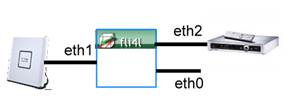
\includegraphics[]{image002}\\
         ~~~~~~~~~~~~~~~~~~~~~~~~~~~~~~~~~~~~~~~~~~~~Interface-LAN
         \caption{fli4l avec la configuration IPTV}
         \label{fig:iptvconfig}
         \end{figure}
      }
\end{itemize}

\subsubsection{Configuration du VLAN}

Tout d'abord~: l'OPT\_IGMP ne dépend pas du VLAN. Le VLAN est plutôt utilisé par Deutsche
Telekom pour le VDSL et doit être supporté par le routeur. Si le VLAN est nécessaire pour
d'autres fournisseurs Internet (Arcor, Alice, etc ..), la configuration est actuelle au-delà
de mes connaissances.

Pour que Internet fonctionne avec le VDSL 25/50 de T-Home, la carte réseau qui est connectée
au modem VDSL doit être configuré comme une interface VLAN.

\vspace{3mm}
\emph{Une note pour ceux qui ont seulement le 'DSL normal', c'est à dire ADSL, ADSL2,
	ADSL2+~: le VLAN est nécessaire uniquement avec le VDSL, mais pas avec le 'DSL normal'.
	La configuration du VLAN ne doit pas être installé avec l'utilisation du 'DSL normal'.}
\vspace{3mm}

Si vous utilisez deux lien VLAN (voir ci-dessus) le trafic se répartit comme ceci~:

\begin{itemize}
   \item{VLAN ID7~: Trafic-Internet}
   \item{VLAN ID8~: Trafic-IPTV Multicast}
\end{itemize}

Donc, le trafic Internet fonctionne indépendamment du trafic IPTV. La principale différence,
il est nécessaire d'utiliser le VLAN ID7 pour les accès entrant PPPoE. Le VLAN ID8 est fournie
par un serveur DHCP sans accès entrant. Dans cette architecture, il n'y a pas de redémarrage
forcé après 24 heures.\\ 

Pour le VLAN la configuration suivante est requise (la carte réseau est indiquée à la section
configuration du matériel)~:\\

\noindent \textbf{advanced\_networking.txt}

\begin{example}
\begin{verbatim}
VLAN_DEV_N='2'
VLAN_DEV_1_DEV='eth1’     # interface of VDSL-Modem; example: eth1
                          # in our example 'eth1' connects to the VDSL modem
VLAN_DEV_1_VID='7         # ID7 to support VLAN for internet
VLAN_DEV_2_DEV='eth1’     # interface of VDSL modem; example: eth1
VLAN_DEV_2_VID='8’        # ID8 to support VLAN for IPTV
\end{verbatim}
\end{example}

\noindent La carte réseau virtual eth1.7 doit être paramétré dans le fichier de configuration DSL~:\\

\noindent \textbf{dsl.txt}

\begin{example}
\begin{verbatim}
PPPOE_ETH='eth1.7'        # eth<number of the card connecting the vdsl modem>.7'
                          # i.e. 'eth1.7'
\end{verbatim}
\end{example}

\noindent Pour la carte réseau virtual eth1.8 vous aurez besoin d'un client\_dhcp, car le VLAN ID8
est configuré par un serveur DHCP sans accès entrant.\\

\noindent \textbf{dhcp\_client}

\begin{example}
\begin{verbatim}
OPT_DHCP_CLIENT='yes'
DHCP_CLIENT_TYPE='dhcpcd'
DHCP_CLIENT_INTERFACES='IP_NET_3_DEV' # listen on interface eth1.8
DHCP_CLIENT_USEPEERDNS='no'
DHCP_CLIENT_HOSTNAME=''
\end{verbatim}
\end{example}

Depuis la v3.3 de fli4l, on ne peut plus définir l'interface avec cette valeur \texttt{eth1.8},
mais vous devez utiliser \texttt{IP\_NET\_x\_DEV} pour définir l'interface depuis le fichier
base.txt; Ici \texttt{IP\_NET\_3\_DEV}.\\

\noindent Facultatif~:\\
Si la carte réseau que vous utilisez a des problèmes avec la taille du MTU, vous pouvez là régler
dans la variable DEV\_MTU. Pendant les testes, la carte Intel Pro/100 (e100) et la 3-Com ont montrées
aucun problème, d'autres utilisateurs ont signalés des problème avec la carte 3Com '3c59x', ils ont
modifiés la valeur MTU à 1496.

\begin{example}
\begin{verbatim}
DEV_MTU_1=''              # Adjust MTU size of NIC on VDSL-Modem
                          # Example: DEV_MTU_1='eth1 1496'
\end{verbatim}
\end{example}

Les fichiers de configuration base.txt et dns\_dhcp.txt doivent être modifiées, comme décrit dans
le chapitre suivant.\\

\subsubsection{Configuration de la carte réseau supplémentaire pour l'IPTV}

Vous devez configuré base.txt et dns\_dhcp.txt pour paramétrer la deuxième carte réseau et le VLAN.\\

\noindent Paramètrage de la deuxième carte réseau pour l'IPTV~:\\

\begin{example}
\begin{verbatim}
NET_DRV_N='2'
NET_DRV_1='via-rhine'     # 1. NIC interface for LAN
NET_DRV_2='3c59x'         # 2. NIC – here 3Com for IPTV SetTopBox
\end{verbatim}
\end{example}

Maintenant nous devons spécifier la plage d'adressage pour la deuxième carte réseau. Nous allons utiliser
pour le réseau local 192.168.2.0/24 et 192.168.3.0/24 pour la deuxième carte réseau. Nous avons besoin
également de paramétrer les cartes virtuelle pour eth1.7 et eth1.8~:\\

\begin{example}
\begin{verbatim}
IP_NET_N='4'
IP_NET_1='192.168.2.1/24'           # home/office LAN
IP_NET_1_DEV='eth0'
IP_NET_2='192.168.3.1/24'           # iptv LAN
IP_NET_2_DEV='eth2'
IP_NET_3='dhcp'                     # dhcp client - IP via dhclient
IP_NET_3_DEV='eth1.8'
IP_NET_3_MAC='00:40:63:da:cf:32'    # new MAC (not the MAC of eth1)
IP_NET_4='dhcp'                     # eth1.7 connecting to the modem
IP_NET_4_DEV='eth1.7'
IP_NET_4_MAC='00:40:63:da:cf:33'    # new MAC (not the MAC of eth1)
\end{verbatim}
\end{example}

Il est important de changer les adresses MAC pour eth1.7 et eth1.8, elles ne doivent pas coïncider
avec eth1, sinon - selon le réseau VDSL - il peut éventuellement se produire des perturbations
après la déconnexion forcée.

Pour que la nouvelle carte réseau puisse accéder à Internet, bien sûr, tout comme pour la première
carte réseau. Ces paramètres supplémentaires sont nécessaires~: \\

\begin{example}
\begin{verbatim}
PF_INPUT_1='IP_NET_1 ACCEPT'
PF_INPUT_2='IP_NET_2 ACCEPT'
PF_INPUT_3='any 224.0.0.0/4 ACCEPT'
[...]
PF_FORWARD_3='any 224.0.0.0/4 ACCEPT'
PF_FORWARD_5='IP_NET_1 ACCEPT'
PF_FORWARD_6='IP_NET_2 ACCEPT'
[...]
PF_POSTROUTING_1='IP_NET_1 MASQUERADE'
PF_POSTROUTING_2='IP_NET_2 MASQUERADE'
\end{verbatim}
\end{example}

Pour que cela fonctionne vous devez paramétrez l'adressage DHCP dynamique sur la carte réseau IPTV,
pour  accéder à la Set-Top Box (ou décodeur) et lui donner un nom. Les paramètres suivants dans
le dns\_dhcp.txt sont nécessaires~: \\

\begin{example}
\begin{verbatim}
HOST_10_NAME='igmp'
HOST_10_IP4='192.168.3.1'
HOST_11_NAME='iptv'
HOST_11_IP4='192.168.3.4'
HOST_11_MAC='00:D0:E0:93:49:34'         # MAC Adr T-Home X300T
[...]
DHCP_RANGE_2_NET='IP_NET_2'
DNSDHCP_RANGE_2_START='192.168.3.10'
DNSDHCP_RANGE_2_END='192.168.3.20'
DNSDHCP_RANGE_2_DNS_SERVER1=''
DNSDHCP_RANGE_2_DNS_SERVER2=''
DNSDHCP_RANGE_2_NTP_SERVER=''
DNSDHCP_RANGE_2_GATEWAY=''
\end{verbatim}
\end{example}

Après avoir configuré la nouvelle carte réseau, il est judicieux de tester l'accès Internet
avec un PC connecté au routeur. Si vous arrivez à vous connecté, la seconde carte réseau sera
configuré correctement.

\subsubsection{Fonctions de l'IGMP}

Lors du démarrage du routeur fli4l les paramètres du fichier de configuration proxy.txt sont
écrit dans le fichier /etc/igmpproxy.conf, ils sont ensuite lu lors du démarrage du proxy IGMP.

Contrairement aux versions antérieures le paquetage opt\_igmp est lancé au démarrage, il est
exécute aussi longtemps que la connexion Internet physique est disponible. Le proxy IGMP n'est
pas affectée par la déconnexion forcé après 24 heures ou par la connexion/déconnexion manuel
de l'accés Internet.

\subsubsection{Configuration de l'IGMP}

\begin{description}

\config{OPT\_IGMPPROXY}{OPT\_IGMPPROXY}{}

Si vous indiquez \var{'yes'}, vous activez le proxy IGMP. avec \var{'no'} vous déactivez
l'ensemble du paquetage.

\config{IGMPPROXY\_DEBUG}{IGMPPROXY\_DEBUG}{IGMPPROXYDEBUG}

Si vous indiquez \var{'yes'} les messages du proxy IGMP sont envoyés à syslog.

\config{IGMPPROXY\_DEBUG2}{IGMPPROXY\_DEBUG2}{IGMPPROXYDEBUG2}

Si vous indiquez \var{'yes'} vous pouvez augmenter le niveau des messages du proxy IGMP.

\config{IGMPPROXY\_QUICKLEAVE\_ON}{IGMPPROXY\_QUICKLEAVE\_ON}{IGMPPROXYQUICKLEAVEON}

Avec Quickleave vous pouvez abaisser la charge de la liaison montante. Si vous avez indiqué
\var{'yes'}, le multicast sera arrêté plus rapidement après un changement de canal et la charge
de la liaison décendante sera réduite par le proxy IGMP, il se comporte comme un récepteur.

Si vous utilisez deux décodeurs et qu'il sont sur le même canal, il peut arriver (avec
l'activation de Quickleave) que le programme soit interrompu sur l'un des décodeurs, vous
devez alors changer le programme. Si vous utilisez un seule décodeur Quickleave peut être
activé en toute sécurité.

\begin{example}
\begin{verbatim}
IGMPPROXY_QUICKLEAVE_ON='yes'      # activate Quickleave mode
                                   # yes or no; Default: yes
\end{verbatim}
\end{example}

\config{IGMPPROXY\_UPLOAD\_DEV}{IGMPPROXY\_UPLOAD\_DEV}{IGMPPROXYUPLOADDEV}

Pour le fonctionnement de l'IPTV avec le proxy IGMP vous avez besoin d'une interface avec
une liaison montante et décendante. L'interface de la liaison montante est l'interface de
la carte réseau qui sera connecté au modem VDSL. Normalement cela doit toujours être la même.

Le transfert de l'IPTV doit se faire sur le lien ID8 avec eth1.8, au lieu de ppp0. Cela doit
être paramétré dans le fichier de configuration.

\begin{example}
\begin{verbatim}
IGMPPROXY_UPLOAD_DEV='eth1.8'      # Upstream interface; Default: ppp0
                                   # eth1.8 for T-Home/VDSL with id7/id8
\end{verbatim}
\end{example}

\config{IGMPPROXY\_DOWNLOAD\_DEV}{IGMPPROXY\_DOWNLOAD\_DEV}{IGMPPROXYDOWNLOADDEV}

L'interface de la liaison décendante (carte réseau pour le décodeur de l'IPTV) dépend de la
configuration matériel. Dans fli4l la deuxième carte réseau eth2 est l'interface pour le décodeur.

\begin{example}
\begin{verbatim}
IGMPPROXY_DOWNLOAD_DEV='eth2'      # Downstream Interface
\end{verbatim}
\end{example}

\config{IGMPPROXY\_ALT\_N}{IGMPPROXY\_ALT\_N}{IGMPPROXYALTN}

Dans cette variable vous indiquez le nombre de plages d'adresse IP pour le flux multicast.

\config{IGMPPROXY\_ALT\_x\_NET}{IGMPPROXY\_ALT\_x\_NET}{IGMPPROXYALTxNET}

Dans la variable IGMPPROXY\_ALT\_NET vous indiquez les adresses IP pour le trafic multicast
provenant de extérieur pour le réseau local, ainsi que l'adresse IP local du décodeur.

\begin{example}
\begin{verbatim}
IGMPPROXY_ALT_N='3'                        # Number of Multicast sources
IGMPPROXY_ALT_1_NET='239.35.0.0/16'        # IPTV streams - always needed
IGMPPROXY_ALT_2_NET='217.0.119.0/24'       # needed for T-Home
IGMPPROXY_ALT_3_NET='193.158.34.0/23'      # needed for T-Home
                                           # before May 2013 '193.158.35.0/24'
# IGMPPROXY_ALT_4_NET='192.168.3.0/24'     # Address range IPTV SetTop-Box/not
                                           # needed anymore
\end{verbatim}
\end{example}

\config{IGMPPROXY\_WLIST\_N}{IGMPPROXY\_WLIST\_N}{IGMPPROXYWLISTN}

Dans cette variable vous indiquez le nombre de listes blanches pour le rapport IGMP.

\config{IGMPPROXY\_WLIST\_x\_NET}{IGMPPROXY\_WLIST\_x\_NET}{IGMPPROXYWLISTxNET}:\newline

Si vous utilisez IGMPv3 toutes les adresses sont regroupées dans un rapport,
(\altlink{http://grinch.itg-em.de/entertain/artikel/zielnetzarchitektur-und-igmpproxy/}). 
Ces adresses seront ensuite complètement ignorées. Cela conduira à un arrêt complet
de tout le trafic multicast par l'émetteur IGMP, en supposant qu'ils ne sont plus
nécessaires. Pour éviter cela, la configuration de listes blanches est utilisée.
Seuls les groupes multicast de cette liste seront épargnés par le WAN.

\begin{example}
\begin{verbatim}
IGMPPROXY_WLIST_N='1'                          # Number of Multicast sources
IGMPPROXY_WLIST_1_NET='239.35.0.0/16'         # IPTV streams - always needed
                                               # see above
\end{verbatim}
\end{example}

\end{description}

\subsubsection{Modification des autres fichiers de configuration}

Avec la révision 32955 il n'est pas nécessaire de paramétrer les règles du pare-feu
pour le proxy IGMP et pour le fux multicast si les règles standard
(\var{PF\_INPUT\_ACCEPT\_DEF='yes'} et \var{PF\_FORWARD\_ACCEPT\_DEF='yes'})
sont activés dans le fichier base.txt, le script de démarrage ajoutera automatiquement
ces règles si la variable \var{OPT\_IGMPPROXY='yes'} est activée.

Il y a deux règles qui sont ajouté dans la chaîne INPUT pour permettre aux messages
entrants d'atteindre le proxy IGMP~:

\begin{example}
\begin{verbatim}
Chain INPUT (policy DROP 0 packets, 0 bytes)
 pkts bytes target   prot opt in   out   source         destination
 [...]
    0     0 ACCEPT   all  --  *    *     0.0.0.0/0      224.0.0.1     \
    /* automatically added for IGMP Proxy */

    0     0 ACCEPT   all  --  *    *     0.0.0.0/0      224.0.0.22    \
    /* automatically added for IGMP Proxy */
 [...]
\end{verbatim}
\end{example}

Vous avez aussi une règle dans la chaîne FORWARD qui permet de transmettre le flux
multicast entrant vers le récepteur de média~:

\begin{example}
\begin{verbatim}
Chain FORWARD (policy DROP 0 packets, 0 bytes)
 pkts bytes target   prot opt in   out   source         destination         
 [...]
    0     0 ACCEPT   all  --  *    *     0.0.0.0/0      239.35.0.0/16  \
    /* automatically added for IPTV streams */
 [..]
\end{verbatim}
\end{example}

Si l'une des règles par défaut n'est pas activée, vous devez au moins paramétrer
et insérer manuellement les règles suivantes.

\begin{example}
\begin{verbatim}
PF_INPUT_x='any 224.0.0.1/32 ACCEPT'
PF_INPUT_x='any 224.0.0.22/32 ACCEPT'
[...]
PF_FORWARD_x='any 239.35.0.0/16 ACCEPT'
\end{verbatim}
\end{example}

\achtung{Remarque~: contrairement aux versions précédentes de la documentation,
	les règles réellement nécessaires ont été écrite pour un réseau limité. Si
	l'IPTV ne fonctionne pas, n'hésitez pas à fournir des informations supplémentaires
	concernant le réseau que vous utilisez.}

\achtung{Important~!
Depuis la fin du mois de mai 2013, Telekom a introduit de nouvelles routes (sans classe prédéfini) pour
améliorer le service (\altlink{http://www.onlinekosten.de/forum/showthread.php?t=116415&page=38}).
Cela est une bonne chose, car plus de 256 émetteurs ou adresses sont utilisables. Maintenant
le serveur DHCP transfére les routes, elles ne sont plus inclusent dans le sous-réseau comme
précédamment. Tant que Telekom ne change pas son sous-réseau du serveur-IPTV (193.158.34.0/23)
la route statique peut être définie vers l'interface vlan8, vous devez faire attention au changement
de celle-ci, sinon le multicast ne fonctionnera plus.}

Solution~: Dans le fichier base.txt, vous devez spécifier une route supplémentaire.

\begin{example}
\begin{verbatim}
IP_ROUTE_N='1'
IP_ROUTE_1='193.158.34.0/23 eth1.8'
\end{verbatim}
\end{example}

% Synchronized to r60625
\subsection{OPT\_STUNNEL - Tunneling Connections Over SSL/TLS}
\configlabel{OPT\_STUNNEL}{OPTSTUNNEL}

The program ``stunnel'' allows to encapsulate connections otherwise unencrypted
in an encrypted SSL/TLS tunnel. This allows safe data exchange over otherwise
insecure cleartext protocols. Due to the possibilities of the SSL/TLS protocol,
various forms of Client/server validation are possible.

\subsubsection{Configuration}
\begin{description}

\config{OPT\_STUNNEL}{OPT\_STUNNEL}{}

This variable activates support for SSL/TLS tunnels.

Default setting: \verb+OPT_STUNNEL='no'+

Example: \verb+OPT_STUNNEL='yes'+

\config{STUNNEL\_DEBUG}{STUNNEL\_DEBUG}{STUNNELDEBUG}

This variable can be set to configure the logging settings for ``stunnel''.
Available settings are ``yes'' (everything is logged), ``no'' (warnings and
errors are logged) or a value between zero and seven indicating the severity of
messages whith zero for highest and seven for lowest severity. The setting ``yes''
corresponds to severity seven, while ``no'' corresponds to severity four.

Default setting: \verb+STUNNEL_DEBUG='no'+

Example 1: \verb+STUNNEL_DEBUG='yes'+

Example 2: \verb+STUNNEL_DEBUG='5'+

\config{STUNNEL\_N}{STUNNEL\_N}{STUNNELN}
This variable configures the number of tunnel instances. Each tunnel instance
``listens'' on a network port ``A'' and connects to another network port ``B''
when a connection is established (may as well be on a different machine), then
forwards all traffic from ``A'' to ``B''. Whether the data, that arrives at
``A'' encrypted via SSL/TLS will be decrypted by ``stunnel'' before forwarding
unencrypted to ``B'' or vice versa is decided by the variable setting in
\jump{STUNNELxCLIENT}{\var{STUNNEL\_x\_CLIENT}}.

Default setting: \verb+STUNNEL_N='0'+

Example: \verb+STUNNEL_N='2'+

\config{STUNNEL\_x\_NAME}{STUNNEL\_x\_NAME}{STUNNELxNAME}

The name of each tunnel. Must be unique for all configured tunnels.

Example: \verb+STUNNEL_1_NAME='imond'+

\config{STUNNEL\_x\_CLIENT}{STUNNEL\_x\_CLIENT}{STUNNELxCLIENT}

This variable configures which parts of the communication are encrypted via
SSL/TLS. There are two options:

\begin{itemize}
\item \emph{Client mode:} The tunnel expects unencrypted data from outside
and sends it encrypted to the other end of the tunnel. This corresponds to
the setting\\
\verb+STUNNEL_x_CLIENT='yes'+.
\item\emph{Server mode:} The tunnel expects data encrypted via SSL/TLS from
outside and will send it decrypted to the other end of the tunnel. This is
equivalent to setting \verb+STUNNEL_x_CLIENT='no'+.
\end{itemize}

Tunnels in client mode hence are particularly suitable for connections ``to
the outside'', i.e. to the (unprotected) Internet because data is encrypted
before leaving the local network. Of course the remote site must offer a server
that expects data encrypted via SSL/TLS. For example an e-mail client in the LAN
only supporting unencrypted POP3 can ``talk'' to a POP3 over SSL service on the
Internet \footnote{see \altlink{http://en.wikipedia.org/wiki/POP3S}}

Tunnels in server mode in reverse are for connections that come ``from the
outside'', i.e. from the (unprotected) Internet providing encrypted data.
If the actual service on the server side is not capable to understand
SSL/TLS the data must be decrypted previously. For example the access to
the fli4l web GUI can be accomplished via HTTP (HTTPS) encrypted via SSL/TLS
by configuring a tunnel on the fli4l receiving HTTP traffic encrypted via
SSL/TLS on port 443, then decrypting the data and forwarding it to the local
web server \texttt{mini\_httpd} listening on port 80.

Configurations for these use cases are presented later.

Example: \verb+STUNNEL_1_CLIENT='yes'+

\config{STUNNEL\_x\_ACCEPT}{STUNNEL\_x\_ACCEPT}{STUNNELxACCEPT}

This determines on which port (and address) the tunnel is ``listening''
for incoming connections. In principle two possibilities exist:

\begin{itemize}
\item The tunnel should listen on \emph{all} addresses (on all interfaces).
Use the setting ``any'' in this case.
\item The tunnel should only listen to defined addresses. Set this with
a reference corresponding to the IP-subnet configured, for example
\var{IP\_NET\_1\_IPADDR} (for IPv4) or \var{IPV6\_NET\_2\_IPADDR} (for IPv6).
\end{itemize}

At the end of the address part the port \emph{must} be added, separated
by a colon (``:'').

Example 1: \verb+STUNNEL_1_ACCEPT='any:443'+

Example 2: \verb+STUNNEL_1_ACCEPT='IP_NET_1_IPADDR:443'+

Example 3: \verb+STUNNEL_1_ACCEPT='IPV6_NET_2_IPADDR:443'+

Please note that using \var{IP\_NET\_x\_IPADDR} resp. \var{IPV6\_NET\_x\_IPADDR}
determines the Layer-3-Protocol (IPv4 or IPv6), the choice here \emph{must}
match with the settings in the variables \var{STUNNEL\_x\_ACCEPT\_IPV4} and
\var{STUNNEL\_x\_ACCEPT\_IPV6}. Hence you may not deactivate IPv6 for the tunnel
by using \verb+STUNNEL_1_ACCEPT_IPV6='no'+ and then listen on an IPv6 address using
\verb+STUNNEL_1_ACCEPT='IPV6_NET_2_IPADDR:443'+ or vice versa by using
(\verb+STUNNEL_1_ACCEPT_IPV4='no'+ and \var{IP\_NET\_x\_IPADDR}).
Furthermore, the meaning of ``any'' depends on the Layer 3 protocols activated
(IPv4 or IPv6): of course, the tunnel only listens on addresses belonging to the
Layer-3-Protocols activated via \var{STUNNEL\_x\_ACCEPT\_IPV4} and
\var{STUNNEL\_x\_ACCEPT\_IPV6}.

\config{STUNNEL\_x\_ACCEPT\_IPV4}{STUNNEL\_x\_ACCEPT\_IPV4}{STUNNELxACCEPTIPV4}

This variable controls if the IPv4 protocol is used for \emph{incoming} connections
to the tunnel. Typically this is the case and this variable should be set to ``yes''
while ``no'' ensures that the tunnel only accepts incoming IPv6 connections. However,
this requires a valid IPv6 configuration (refer to the documentation for the ipv6
package for more information).

Default setting: \verb+STUNNEL_x_ACCEPT_IPV4='yes'+

Example: \verb+STUNNEL_1_ACCEPT_IPV4='no'+

\config{STUNNEL\_x\_ACCEPT\_IPV6}{STUNNEL\_x\_ACCEPT\_IPV6}{STUNNELxACCEPTIPV6}

Like in \var{STUNNEL\_x\_ACCEPT\_IPV4} this variable controls whether the IPv6
protocol is used for incoming connections to the tunnel. Typically this is the case
if you use the the general IPv6 protocol by using \verb+OPT_IPV6='yes'+. Setting
``no'' here ensures that the tunnel only accepts incoming IPv4 connections.

Default setting: \verb+STUNNEL_x_ACCEPT_IPV6=<Values from OPT_IPV6>+

Example: \verb+STUNNEL_1_ACCEPT_IPV6='no'+

\config{STUNNEL\_x\_CONNECT}{STUNNEL\_x\_CONNECT}{STUNNELxCONNECT}

Sets the target of the SSL/TLS tunnel. There are basically three possibilities and all
must have the port  appended, separated by a colon (``:''):

\begin{itemize}
\item A numeric IPv4- or IPv6 address

Example 1: \verb+STUNNEL_1_CONNECT='192.0.2.2:443'+

\item The DNS name of an internal host

Example 2: \verb+STUNNEL_1_CONNECT='@webserver:443'+

\item The DNS name of an external host

Example 3: \verb+STUNNEL_1_CONNECT='@www.example.com:443'+
\end{itemize}

If an internal host is entered with both IPv4 and IPv6 address,
the IPv4 address is preferred. If an external host is entered with both
IPv4 and IPv6 address, then the Layer 3 protocol used depends on
which address is first returned by the DNS resolver.

\config{STUNNEL\_x\_OUTGOING\_IP}{STUNNEL\_x\_OUTGOING\_IP}{STUNNELxOUTGOINGIP}

With this optional variable, the \emph{local} address for the
\emph{outgoing} connection of the tunnel can be set. This is only
useful if the target of the tunnel can be reached over multiple interfaces
(routes), i.e. if two concurrent Internet connections are used.
Normally, this variable must not be set.

Example: \verb+STUNNEL_1_OUTGOING_IP='IP_NET_1_IPADDR'+

\config{STUNNEL\_x\_DELAY\_DNS}{STUNNEL\_x\_DELAY\_DNS}{STUNNELxDELAYDNS}

If this optional variable is set to ``yes'', an external DNS name used in
\var{STUNNEL\_x\_CONNECT} will not be converted to an address until the
\emph{outbound} tunnel is established, meaning the point when the first client
has connected locally with the incoming side of the tunnel. This is useful if
the target of the tunnel is a computer that can only be reached through a
dynamic DNS name and the address behind the name changes frequently, or if
an active dialin when starting ``stunnel'' should be prevented.

Default setting: \verb+STUNNEL_x_DELAY_DNS='no'+

Example: \verb+STUNNEL_1_DELAY_DNS='yes'+

\config{STUNNEL\_x\_CERT\_FILE}{STUNNEL\_x\_CERT\_FILE}{STUNNELxCERTFILE}

This variable contains the file name of the certificate for the tunnel to be used.
For server mode tunnels (\verb+STUNNEL_x_CLIENT='no'+) this is the server
certificate that the client validates against a ``Certificate Authority'' (CA)
if necessary. For client mode tunnels (\verb+STUNNEL_x_CLIENT='yes'+)
this is a (usually optional) client certificate that is validated by the
server against a CA if necessary.

The certificate must be provided in the so-called PEM format and must be saved below\\
\texttt{<config-directory>/etc/ssl/stunnel/}. Only the file name must be stored
in this variable, not the path.

For a server mode tunnel the certificate is mandatory!

Example: \verb+STUNNEL_1_CERT_FILE='myserver.crt'+

\config{STUNNEL\_x\_CERT\_CA\_FILE}{STUNNEL\_x\_CERT\_CA\_FILE}{STUNNELxCERTCAFILE}

This variable contains the file name of the CA certificate to be used for the
validation of the certificate of the remote station. Typically clients validate
the server's certificate, vice versa however, is also possible. For details on
the validation please refer to the description of the variable \jump{STUNNELxCERTVERIFY}
{\var{STUNNEL\_x\_CERT\_VERIFY}}.

The certificate must be provided in the so-called PEM format and must be saved below\\
\texttt{<config-directory>/etc/ssl/stunnel/}. Only the file name must be stored
in this variable, not the path.

Example: \verb+STUNNEL_1_CERT_CA_FILE='myca.crt'+

\config{STUNNEL\_x\_CERT\_VERIFY}{STUNNEL\_x\_CERT\_VERIFY}{STUNNELxCERTVERIFY}

This variable controls the validation of the certificate of the remote station.
There are five options possible:

\begin{itemize}
\item \emph{none:} The certificate of the remote station is not validated at all.
In this case the variable \var{STUNNEL\_x\_CERT\_CA\_FILE} is empty.

\item \emph{optional:} If the remote station provides a certificate it is checked
against the CA certificate configured using the variable \var{STUNNEL\_x\_CERT\_CA\_FILE}.
If the remote station does \emph{not} provide a certificate this is not an error and the
connection is still accepted. This setting is only useful for server mode tunnel because
the client tunnel \emph{always} obtain a certificate from the server.

\item \emph{onlyca:} The certificate of the remote station is validated against
the CA certificate configured in the variable \var{STUNNEL\_x\_CERT\_CA\_FILE}.
If the remote station does not provide a certificate or it does not match the
configured CA, the connection is rejected. This is useful when a private CA is used,
as then all potential peers are know.

\item \emph{onlycert:} The certificate of the remote station is compared with
the certificate configured in the variable \var{STUNNEL\_x\_CERT\_CA\_FILE}.
It is \emph{not} checked against a CA certificate, but it will be ensured that
the remote station sends \emph{exactly} the matching (server or client) certificate.
The file referenced with the help of the variable \var{STUNNEL\_x\_CERT\_CA\_FILE}
in this case does not contain a CA certificate, but a host certificate. This setting
ensures that really only a fixed and known peer may connect (server tunnel) or
a connection to only a known peer (client tunnel) is established. This is useful for
peer-to-peer connections between hosts both under your control, but for which no
own CA is used.

\item \emph{both:} The certificate of the remote station is compared  with the
certificate configured by the help of the variable \var{STUNNEL\_x\_CERT\_CA\_FILE}
\emph{and} it is also ensured that it matches a CA certificate. The file referenced
by the help of the variable \var{STUNNEL\_x\_CERT\_CA\_FILE} in this case contains
\emph{both} a CA \emph{and} a host certificate. It is therefore a combination of
the settings \emph{onlycert} and \emph{onlyca}. In comparison to the setting
\emph{onlycert} connections with expired CA certificate will be rejected (even if the
certificate of the peer matches).

\end{itemize}

Default setting: \verb+STUNNEL_x_CERT_VERIFY='none'+

Example: \verb+STUNNEL_1_CERT_VERIFY='onlyca'+

\end{description}

\subsubsection{Use Case 1: Accessing the fli4l-WebGUI via SSL/TLS}

This example enhances the fli4l-WebGUI with SSL/TLS access.

\begin{example}
\begin{verbatim}
OPT_STUNNEL='yes'
STUNNEL_N='1'

STUNNEL_1_NAME='http'
STUNNEL_1_CLIENT='no'
STUNNEL_1_ACCEPT='any:443'
STUNNEL_1_ACCEPT_IPV4='yes'
STUNNEL_1_ACCEPT_IPV6='yes'
STUNNEL_1_CONNECT='127.0.0.1:80'
STUNNEL_1_CERT_FILE='server.pem'
STUNNEL_1_CERT_CA_FILE='ca.pem'
STUNNEL_1_CERT_VERIFY='none'
\end{verbatim}
\end{example}

\subsubsection{Use Case 2: Controlling two remote
fli4l routers via imonc secured by SSL/TLS}

The known weaknesses of the imonc/imond protocol for WAN connections (sending
passwords in clear text) are bypassed with this example. (The LAN connection to
the tunnel of course is vulnerable!)\\

Configuration of the local fli4l in LAN (client tunnel):
\begin{example}
\begin{verbatim}
OPT_STUNNEL='yes'
STUNNEL_N='2'

STUNNEL_1_NAME='remote-imond1'
STUNNEL_1_CLIENT='yes'
STUNNEL_1_ACCEPT='any:50000'
STUNNEL_1_ACCEPT_IPV4='yes'
STUNNEL_1_ACCEPT_IPV6='yes'
STUNNEL_1_CONNECT='@remote1:50000'
STUNNEL_1_CERT_FILE='client.pem'
STUNNEL_1_CERT_CA_FILE='ca+server1.pem'
STUNNEL_1_CERT_VERIFY='both'

STUNNEL_2_NAME='remote-imond2'
STUNNEL_2_CLIENT='yes'
STUNNEL_2_ACCEPT='any:50001'
STUNNEL_2_ACCEPT_IPV4='yes'
STUNNEL_2_ACCEPT_IPV6='yes'
STUNNEL_2_CONNECT='@remote2:50000'
STUNNEL_2_CERT_FILE='client.pem'
STUNNEL_2_CERT_CA_FILE='ca+server2.pem'
STUNNEL_2_CERT_VERIFY='both'
\end{verbatim}
\end{example}

Configuration of the first remote fli4l (server tunnel):
\begin{example}
\begin{verbatim}
OPT_STUNNEL='yes'
STUNNEL_N='1'

STUNNEL_1_NAME='remote-imond'
STUNNEL_1_CLIENT='no'
STUNNEL_1_ACCEPT='any:50000'
STUNNEL_1_ACCEPT_IPV4='yes'
STUNNEL_1_ACCEPT_IPV6='yes'
STUNNEL_1_CONNECT='127.0.0.1:5000'
STUNNEL_1_CERT_FILE='server1.pem'
STUNNEL_1_CERT_CA_FILE='ca+client.pem'
STUNNEL_1_CERT_VERIFY='both'
\end{verbatim}
\end{example}

Configuration of the second remote fli4l (server tunnel):
\begin{example}
\begin{verbatim}
OPT_STUNNEL='yes'
STUNNEL_N='1'

STUNNEL_1_NAME='remote-imond'
STUNNEL_1_CLIENT='no'
STUNNEL_1_ACCEPT='any:50000'
STUNNEL_1_ACCEPT_IPV4='yes'
STUNNEL_1_ACCEPT_IPV6='yes'
STUNNEL_1_CONNECT='127.0.0.1:5000'
STUNNEL_1_CERT_FILE='server2.pem'
STUNNEL_1_CERT_CA_FILE='ca+client.pem'
STUNNEL_1_CERT_VERIFY='both'
\end{verbatim}
\end{example}

A connection to the remote ``imond'' is established by initiating a connection
to the local fli4l on port 50000 (first remote fli4l) resp. 50001 (second remote
fli4l). This fli4l then connects via SSL/TLS-Tunnel to each of the remote fli4l's
which in turn forward their data over a third (host internal) connection to the
remote ``imond'' in the end. The settings of the validation ensure that each fli4l
only accepts the other fli4l as the connecting counterpart.



\listoffigures
\listoftables
\printindex

\end{document}

